\documentclass{article}
\usepackage[utf8]{inputenc} %кодировка
\usepackage[T2A]{fontenc}
\usepackage[english,russian]{babel} %русификатор 
\usepackage{mathtools} %библиотека матеши
\usepackage[left=1cm,right=1cm,top=2cm,bottom=2cm,bindingoffset=0cm]{geometry} %изменение отступов на листе
\usepackage{amsmath}
\usepackage{graphicx} %библиотека для графики и картинок
\graphicspath{}
\DeclareGraphicsExtensions{.pdf,.png,.jpg}
\usepackage{subcaption}
\usepackage{pgfplots}
\usepackage{float}
\usepackage{listings}


\lstset{
    numbers=left,            % Нумерация строк слева
    numberstyle=\tiny,       % Размер шрифта для номеров строк
    stepnumber=1,            % Нумеровать каждую строку
    numbersep=5pt,           % Расстояние между номерами и кодом
    backgroundcolor=\color{white},  % Цвет фона
    showspaces=false,        % Не показывать пробелы
    showstringspaces=false,  % Не показывать пробелы в строках
    showtabs=false,          % Не показывать табуляцию
    frame=single,            % Рамка вокруг кода
    tabsize=2,               % Размер табуляции
    breaklines=true,         % Автоматический перенос строк
    breakatwhitespace=true   % Переносить строки только по пробелам
}


\begin{document}
% НАЧАЛО ТИТУЛЬНОГО ЛИСТА
\begin{center}
    \Large
    Федеральное государственное автономное \\
    образовательное учреждение высшего образования \\ 
    «Научно-образовательная корпорация ИТМО»\\
    \vspace{0.5cm}
    \large
    Факультет программной инженерии и компьютерной техники \\
    Направление подготовки 09.03.04 Программная инженерия \\
    \vspace{1cm}
    \Large
    \textbf{Отчёт по лабораторной работе №3} \\
        По дисциплине «Распределённые системы хранения данных» ( семестр 6)\\
    \large
    \vspace{8cm}

    \begin{minipage}{.33\textwidth}
    \end{minipage}
    \hfill
    \begin{minipage}{.4\textwidth}
    
        \textbf{Студент}: \vspace{.1cm} \\
        \ Дениченко Александр P3312\\
        \textbf{Практик}:  \\
        \ Осипов Святослав
    \end{minipage}
    \vfill
Санкт-Петербург\\ 2025 г.
\end{center}
\pagestyle{empty}
% КОНЕЦ ТИТУЛЬНОГО ЛИСТА 
\newpage
\pagestyle{plain}

\section*{Задание}
Цель работы - настроить процедуру периодического резервного копирования базы данных, сконфигурированной в ходе выполнения лабораторной работы №2, а также разработать и отладить сценарии восстановления в случае сбоев.

Узел из предыдущей лабораторной работы используется в качестве основного. Новый узел используется в качестве резервного. Учётные данные для подключения к новому узлу выдаёт преподаватель. В сценариях восстановления необходимо использовать копию данных, полученную на первом этапе данной лабораторной работы.

\section*{Этап 1. Резервное копирование}
Настроить резервное копирование с основного узла на резервный следующим образом:
Периодические полные копии с помощью SQL Dump.
По расписанию (cron) раз в сутки, методом SQL Dump с сжатием. Созданные архивы должны сразу перемещаться на резервный хост, они не должны храниться на основной системе. Срок хранения архивов на резервной системе - 4 недели. По истечении срока хранения, старые архивы должны автоматически уничтожаться.
\\ \\
Изначально сделаем донастройку конфигураций прежней базы данных.
\begin{lstlisting}[caption={kitty}, label={lst:example}]
    docker create --name postgres-cont-1 -e POSTGRES_PASSWORD=root -p 9193:9193 postgres
\end{lstlisting}

\begin{lstlisting}[caption={kitty}, label={lst:example}]
    docker start postgres-cont-1 
    docker exec -it postgres-cont-1 /bin/bash
\end{lstlisting}

Изменение некоторых настроек разрешений
\begin{lstlisting}[caption={postgresql.conf}, label={lst:example}]
    listen_addresses = '*'
\end{lstlisting}
\begin{lstlisting}[caption={pg\_hba.conf}, label={lst:example}]
    host    all    all    0.0.0.0/0    scram-sha-256
\end{lstlisting}
Подключение к первому узлу теперь выглядит следующим образом.
\begin{lstlisting}[caption={kitty}, label={lst:example}]
    psql -h 127.0.0.1 -p 9193 -U postgres -d postgres 
    psql -h 127.0.0.1 -p 9193 -U postgres -d fatrednews     
    psql -h 127.0.0.1 -p 9193 -U fatreduser -d fatrednews 
\end{lstlisting}

\textbf{postgres - root}

\textbf{fatreduser - changeMe}
\\ \\
Табличные пространства из прошлой лабы

\begin{lstlisting}[caption={kitty}, label={lst:example}]
    List of tablespaces
    Name    |  Owner   |         Location          | Access privileges | Options |  Size   | Description 
    ------------+----------+---------------------------+-------------------+---------+---------+-------------
    pg_default | postgres |                           |                   |         | 22 MB   | 
    pg_global  | postgres |                           |                   |         | 565 kB  | 
    sgk31      | postgres | /var/lib/postgresql/sgk31 |                   |         | 0 bytes | 
    yrp30      | postgres | /var/lib/postgresql/yrp30 |                   |         | 0 bytes | 
    yva58      | postgres | /var/lib/postgresql/yva58 |                   |         | 0 bytes | 
    (5 rows)
\end{lstlisting}


Создан узел для хранения бэкапов

\begin{lstlisting}[caption={kitty}, label={lst:example}]
    docker create --name postgres-backup -e POSTGRES_PASSWORD=root -p 9194:9193 postgres
    docker network connect pg_backup_network postgres-backup
    docker restart postgres-backup
\end{lstlisting}

Добавлены утилиты на резервном узле и на основном
\begin{lstlisting}[caption={kitty}, label={lst:example}]
    apt-get install -y cron openssh-client openssh-server gzip
\end{lstlisting}

Была сделана сеть докер для обмена

\begin{lstlisting}[caption={kitty}, label={lst:example}]
    docker network create --driver bridge postgres-backup-net 
    docker network connect postgres-backup-net postgres-cont-1 postgres-backup
    docker restart postgres-cont-1 postgres-backup
\end{lstlisting}

Добавим конфиг в сервер 
\begin{lstlisting}[caption={kitty}, label={lst:example}]
    echo "PermitRootLogin yes" >> /etc/ssh/sshd_config
    chmod 700 /root/.ssh
    mkdir -p /run/sshd
    chmod 755 /run/sshd
    service ssh start
\end{lstlisting}

Добавлены ключи для упрощения обмена данными на основном сервере
\begin{lstlisting}[caption={kitty}, label={lst:example}]
    ssh-keygen -t rsa -b 4096
    cat ~/.ssh/id_rsa.pub 
\end{lstlisting}

И добавили ключи в резервный узел
\begin{lstlisting}[caption={kitty}, label={lst:example}]
    vim ~/.ssh/authorized_keys ....
\end{lstlisting}

Настройка скрипта для копирования
\begin{lstlisting}[caption={kitty}, label={lst:example}]
#!/bin/bash

PG_USER="postgres"
BACKUP_DIR="/tmp/backups"
REMOTE_HOST="postgres-backup"
REMOTE_DIR="/backups"
TIMESTAMP=$(date +%Y%m%d_%H%M%S)
BACKUP_FILE="full_backup-$TIMESTAMP.tar.gz"
LOG_FILE="/tmp/backup_log.txt"
PGDATA="/var/lib/postgresql/data"

echo "Starting backup: $TIMESTAMP" >> $LOG_FILE

mkdir -p $BACKUP_DIR
BACKUP_TEMP_DIR="$BACKUP_DIR/backup_$TIMESTAMP"
mkdir -p "$BACKUP_TEMP_DIR"

if pg_dumpall -p 9193 -U $PG_USER > "$BACKUP_TEMP_DIR/full_backup.sql"; then
    echo "Database dump created successfully" >> $LOG_FILE
else
    echo "Database dump failed" >> $LOG_FILE
    exit 1
fi

cp "$PGDATA/postgresql.conf" "$BACKUP_TEMP_DIR/" || echo "Failed to copy postgresql.conf" >> $LOG_FILE
cp "$PGDATA/pg_hba.conf" "$BACKUP_TEMP_DIR/" || echo "Failed to copy pg_hba.conf" >> $LOG_FILE

mkdir -p "$BACKUP_TEMP_DIR/pg_tblspc"
cp -r "$PGDATA/pg_tblspc/"* "$BACKUP_TEMP_DIR/pg_tblspc/" 2>/dev/null || echo "No tablespaces found or failed to copy" >> $LOG_FILE


for tblspc in "$PGDATA/pg_tblspc/"*; do
    if [ -L "$tblspc" ]; then
        REAL_PATH=$(readlink -f "$tblspc")
        mkdir -p "$BACKUP_TEMP_DIR/tblspc_data/$(basename "$tblspc")"
        cp -r "$REAL_PATH/"* "$BACKUP_TEMP_DIR/tblspc_data/$(basename "$tblspc")/"
    fi
done

tar -czf "$BACKUP_DIR/$BACKUP_FILE" -C "$BACKUP_TEMP_DIR" .

if scp "$BACKUP_DIR/$BACKUP_FILE" "$REMOTE_HOST:$REMOTE_DIR/"; then
    echo "Backup transferred successfully" >> $LOG_FILE
else
    echo "Transfer failed" >> $LOG_FILE
    exit 1
fi

rm -rf "$BACKUP_TEMP_DIR"
rm "$BACKUP_DIR/$BACKUP_FILE"

echo "Backup script completed" >> $LOG_FILE
\end{lstlisting}

Сама настройка для автоматизации на основном хосте
\begin{lstlisting}[caption={kitty}, label={lst:example}]
    crontab -e 
    */1 * * * * /backup.sh
    cron
\end{lstlisting}

Настройка для автоматизации на доп хосте
\begin{lstlisting}[caption={kitty}, label={lst:example}]
    crontab -e 
    */2 * * * * /cleanup_dumps.sh
    cron
\end{lstlisting}

\section*{Расчет объема резервных копий через месяц}

Исходные данные:

- Средний объем новых данных в БД за сутки: 950 МБ.

- Средний объем измененных данных за сутки: 150 МБ.

- Период хранения резервных копий: 4 недели (28 дней).
\\
Предположения:

1. Бэкап делается полностью (включает все данные, а не только новые или измененные).

2. Измененные данные не увеличивают общий объем бэкапа, так как они уже входят в полную копию.

3. Объем БД увеличивается со временем за счет новых данных.
\\
Каждый день создается новая полная резервная копия.  
Объем бэкапа на n-й день равен всему объему базы данных на тот момент.

Объем базы через n дней можно выразить как:

\[
V(n) = V_0 + 950 \times n
\]

Где:

- \( V_0 \) — начальный объем базы (пусть 0 для расчета за 1 месяц),

- 950 — рост базы в день.
\\ \\
Общий объем всех бэкапов за 28 дней:
\[
V_{\text{total}} = \sum_{n=1}^{28} (950 \times n)
\]

---

Рассчитаем сумму:

\[
V_{\text{total}} = 950 \times (1 + 2 + ... + 28)
\]

Сумма арифметической прогрессии:
\[
S = \frac{n (n+1)}{2}
\]
Где \( n = 28 \):

\[
S = \frac{28 \times 29}{2} = 406
\]

Подставляем:
\[
V_{\text{total}} = 950 \times 406 = 385 700 \text{ МБ} = 385.7 \text{ ГБ}
\]

\section*{Потеря основного узла}

\begin{lstlisting}[caption={kitty}, label={lst:example}]
#!/bin/bash

PG_USER="postgres"
BACKUP_DIR="/backups"
RESTORE_TEMP_DIR="/tmp/restore_temp"
PGDATA="/var/lib/postgresql/data"
LOG_FILE="/tmp/restore_log.txt"
BACKUP_FILE="$1"  

if [ -z "$BACKUP_FILE" ]; then
    echo "Error: Backup file not specified. Usage: $0 /backups/full_backup-YYYYMMDD_HHMMSS.tar.gz" >> $LOG_FILE
    exit 1
fi

echo "Starting restore: $(date +%Y%m%d_%H%M%S)" >> $LOG_FILE

if pg_ctl -D "$PGDATA" status > /dev/null 2>&1; then
    pg_ctl -D "$PGDATA" stop -m fast || {
        echo "Failed to stop PostgreSQL" >> $LOG_FILE
        exit 1
    }
fi

rm -rf "$PGDATA"/* || {
    echo "Failed to clean PGDATA" >> $LOG_FILE
    exit 1
}

mkdir -p "$RESTORE_TEMP_DIR"
tar -xzf "$BACKUP_FILE" -C "$RESTORE_TEMP_DIR" || {
    echo "Failed to extract backup" >> $LOG_FILE
    exit 1
}

cp "$RESTORE_TEMP_DIR/postgresql.conf" "$PGDATA/" || echo "Failed to restore postgresql.conf" >> $LOG_FILE
cp "$RESTORE_TEMP_DIR/pg_hba.conf" "$PGDATA/" || echo "Failed to restore pg_hba.conf" >> $LOG_FILE

for tblspc in "$RESTORE_TEMP_DIR/pg_tblspc/"*; do
    if [ -f "$tblspc" ]; then
        TBL_ID=$(basename "$tblspc")
        TBL_PATH=$(readlink "$tblspc")
        mkdir -p "$TBL_PATH" || echo "Failed to create tablespace dir $TBL_PATH" >> $LOG_FILE
        ln -s "$TBL_PATH" "$PGDATA/pg_tblspc/$TBL_ID" || echo "Failed to link tablespace $TBL_ID" >> $LOG_FILE
    fi
done

if [ -d "$RESTORE_TEMP_DIR/tblspc_data" ]; then
    for tblspc in "$RESTORE_TEMP_DIR/tblspc_data/"*; do
        TBL_ID=$(basename "$tblspc")
        TBL_PATH=$(readlink "$RESTORE_TEMP_DIR/pg_tblspc/$TBL_ID")
        cp -r "$tblspc/"* "$TBL_PATH/" || echo "Failed to restore tablespace data for $TBL_ID" >> $LOG_FILE
    done
fi

pg_ctl -D "$PGDATA" start || {
    echo "Failed to start PostgreSQL" >> $LOG_FILE
    exit 1
}

psql -U $PG_USER -f "$RESTORE_TEMP_DIR/full_backup.sql" || {
    echo "Failed to restore database" >> $LOG_FILE
    exit 1
}

rm -rf "$RESTORE_TEMP_DIR"

echo "Restore completed successfully" >> $LOG_FILE
\end{lstlisting}


Пример восстановления базы данных
\\ \\
Запуск резервного узла
\begin{lstlisting}[caption={kitty}, label={lst:example}]
    docker exec -it postgres-backup /bin/bash
\end{lstlisting}

Должно быть включено ssh и общая есть у двух контейнеров.
\begin{lstlisting}[caption={kitty}, label={lst:example}]
    service ssh start
\end{lstlisting}

Делаем типо последний бэкап с основного узла перед его выходом из строя
\begin{lstlisting}[caption={kitty}, label={lst:example}]
    root@7f898d3520a8:/# ./backup.sh 
    full_backup-20250401_190056.tar.gz         100%   14KB  30.0MB/s   00:00    
\end{lstlisting}

\end{document}



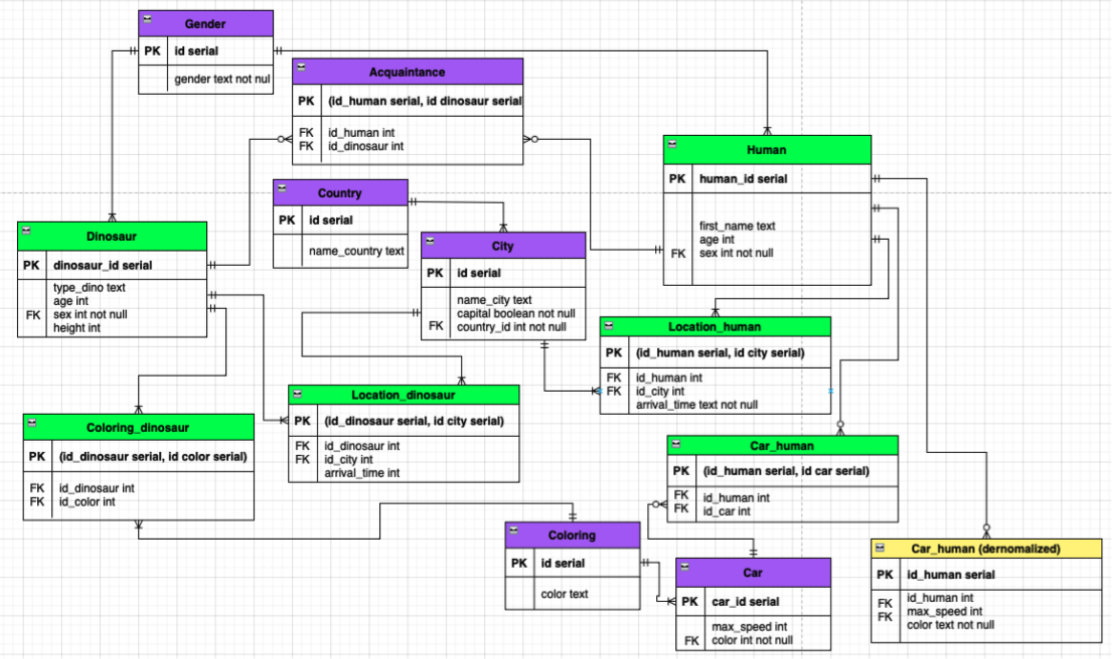
\includegraphics[width=.9\textwidth]{123}

\begin{lstlisting}[caption={kitty}, label={lst:example}]

\end{lstlisting}